%% ================================================================
%% VLA Web Agent — Architecture & Defect-Resolution Report
%% ================================================================
\documentclass[11pt,a4paper]{article}

\usepackage[margin=1in]{geometry}
\usepackage{booktabs}
\usepackage{hyperref}
\usepackage{xcolor}
\usepackage{listings}
\usepackage{amsmath,amssymb}
\usepackage{graphicx}
\usepackage{float}
\usepackage{enumitem}
\usepackage{tikz}
\usepackage{pgfplots}
\pgfplotsset{compat=1.18}
\usetikzlibrary{shapes.geometric,arrows.meta,positioning,fit,
                 calc,decorations.pathreplacing,backgrounds,
                 patterns,matrix}

% Code listing style
\lstdefinestyle{python}{
  language=Python,
  basicstyle=\ttfamily\footnotesize,
  keywordstyle=\color{blue!70!black}\bfseries,
  commentstyle=\color{green!50!black}\itshape,
  stringstyle=\color{red!60!black},
  showstringspaces=false,
  breaklines=true,
  frame=single,
  backgroundcolor=\color{gray!5},
  numbers=left,
  numberstyle=\tiny\color{gray},
  tabsize=4,
}

\definecolor{critical}{RGB}{204,0,0}
\definecolor{significant}{RGB}{204,102,0}
\definecolor{moderate}{RGB}{0,102,204}
\definecolor{improvement}{RGB}{0,153,51}

\title{
  \textbf{VLA Web Agent} \\[4pt]
  \large Architecture \& Defect-Resolution Report
}
\author{Generated by Automated Code Audit}
\date{\today}

\begin{document}
\maketitle
\tableofcontents
\newpage

%% ================================================================
\section{Executive Summary}
%% ================================================================

This report documents the comprehensive audit and resolution of defects in
the Vision-Language-Action (VLA) Web Agent codebase. The agent uses a
fine-tuned Qwen2-VL model with QLoRA to perform autonomous web
navigation via candidate-based element selection.

The audit identified \textbf{19 defects and improvements} across 4
severity levels, all of which have been resolved.

\begin{table}[H]
\centering
\caption{Defect summary by severity}
\begin{tabular}{lccc}
\toprule
\textbf{Severity} & \textbf{Count} & \textbf{Fixed} & \textbf{Files Modified} \\
\midrule
\textcolor{critical}{Critical (C)} & 4 & 4 & 5 \\
\textcolor{significant}{Significant (S)} & 7 & 7 & 7 \\
\textcolor{moderate}{Moderate (M)} & 2 & 2 & 2 \\
\textcolor{improvement}{Improvement (I)} & 6 & 6 & 8 \\
\midrule
\textbf{Total} & \textbf{19} & \textbf{19} & \textbf{12 unique} \\
\bottomrule
\end{tabular}
\end{table}


%% ================================================================
\section{System Architecture}
%% ================================================================

\subsection{Module Structure}

\begin{table}[H]
\centering
\small
\caption{Module inventory}
\begin{tabular}{lll}
\toprule
\textbf{Module} & \textbf{File} & \textbf{Purpose} \\
\midrule
Data Loading     & \texttt{data/mind2web\_loader.py}    & Dataset, candidates, trajectories \\
Prompt Building  & \texttt{models/prompt\_builder.py}    & Chat template construction \\
VLA Model        & \texttt{models/vla\_model.py}         & Qwen2-VL wrapper with QLoRA \\
Action Decoder   & \texttt{models/action\_decoder.py}    & JSON parsing \& validation \\
Candidate Ranker & \texttt{models/candidate\_ranker.py}  & Semantic similarity ranking \\
Task Planner     & \texttt{models/task\_planner.py}      & Subgoal decomposition \\
Uncertainty      & \texttt{models/uncertainty.py}        & Token-level confidence \\
Failure Detector & \texttt{memory/failure\_detector.py}  & Loop \& stale-state detection \\
Browser Env      & \texttt{environment/playwright\_env.py} & Playwright browser control \\
Inference Agent  & \texttt{inference/run\_agent.py}       & End-to-end task execution \\
Training         & \texttt{training/train\_supervised.py} & Multi-stage imitation learning \\
Evaluation       & \texttt{evaluation/evaluate.py}       & Metrics computation \\
Configuration    & \texttt{utils/config.py}              & Dataclass-based configuration \\
\bottomrule
\end{tabular}
\end{table}


\subsection{Candidate-Based Action Format}

The agent uses a candidate-indexed action format. Each DOM element is
assigned a sequential index in the prompt, and the model outputs JSON:

\begin{lstlisting}[style=python]
{"action": "CLICK", "candidate": 3}
{"action": "TYPE", "candidate": 7, "value": "New York"}
{"action": "SCROLL", "direction": "down"}
\end{lstlisting}


%% ================================================================
\section{Training Pipeline}
%% ================================================================

\subsection{Stage 1: Single-Step Imitation}

Stage~1 trains the model on independent \texttt{(state, action)} pairs.
Each sample is processed through the full multimodal pipeline shown in
Figure~\ref{fig:stage1-pipeline}.

\begin{figure}[H]
\centering
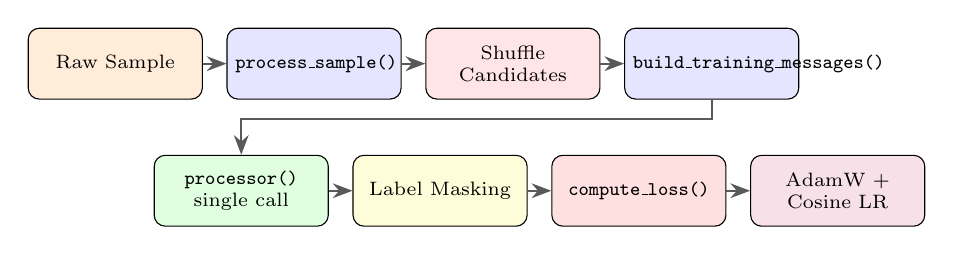
\begin{tikzpicture}[
  block/.style={rectangle, draw, rounded corners=4pt, minimum height=0.9cm,
                minimum width=2.0cm, text centered, font=\scriptsize,
                fill=#1, text width=2.0cm, inner sep=3pt},
  block/.default={blue!10},
  arrow/.style={-{Stealth[length=2.5mm]}, thick, color=gray!70!black},
  node distance=0.3cm
]
  \node[block=orange!15] (raw)  {Raw Sample};
  \node[block, right=of raw] (proc) {\texttt{process\_sample()}};
  \node[block=red!10, right=of proc] (shuf) {Shuffle Candidates};
  \node[block, right=of shuf] (build) {\texttt{build\_training\_messages()}};
  \node[block=green!12, below=0.7cm of raw, xshift=1.6cm] (call) {\texttt{processor()} single call};
  \node[block=yellow!15, right=of call] (mask) {Label Masking};
  \node[block=red!12, right=of mask] (loss) {\texttt{compute\_loss()}};
  \node[block=purple!12, right=of loss] (opt) {AdamW + Cosine LR};

  \draw[arrow] (raw) -- (proc);
  \draw[arrow] (proc) -- (shuf);
  \draw[arrow] (shuf) -- (build);
  \draw[arrow] (build.south) -- ++(0,-0.25) -| (call.north);
  \draw[arrow] (call) -- (mask);
  \draw[arrow] (mask) -- (loss);
  \draw[arrow] (loss) -- (opt);
\end{tikzpicture}
\caption{Stage 1 training pipeline: single-step imitation learning.}
\label{fig:stage1-pipeline}
\end{figure}

Key invariants:
\begin{itemize}[nosep]
  \item Candidates are shuffled \emph{before} building the prompt
        (preventing position bias).
  \item The processor is called \emph{once} for the entire batch ---
        per-sample calls corrupt \texttt{image\_grid\_thw}.
  \item Labels are masked so only the assistant's JSON output
        contributes to the loss.
\end{itemize}


\subsection{Stage 2: Multi-Step Trajectories (C2~Fix)}

\subsubsection{Trajectory Grouping: Before vs After}

The critical C2~defect caused Stage~2 to degenerate into Stage~1.
Figure~\ref{fig:traj-grouping} shows the broken and fixed grouping.

\begin{figure}[H]
\centering
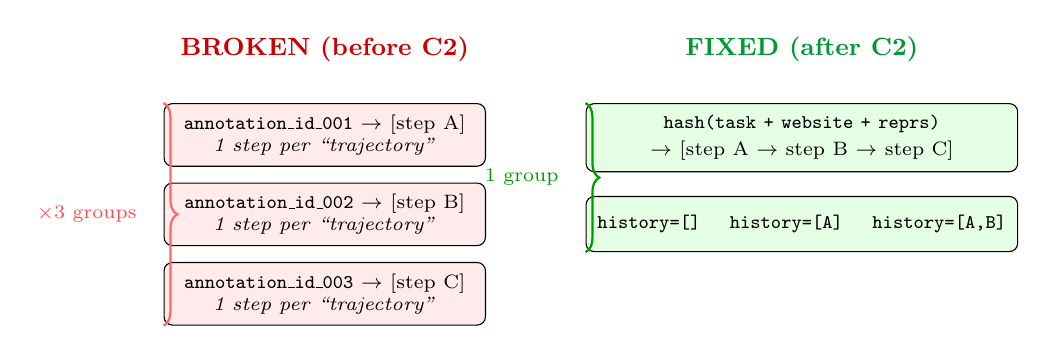
\begin{tikzpicture}[
  box/.style={rectangle, draw, rounded corners=3pt, minimum height=0.7cm,
              text centered, font=\scriptsize, inner sep=4pt},
  title/.style={font=\small\bfseries},
  arrow/.style={-{Stealth[length=2mm]}, thick},
  node distance=0.3cm
]
  % ── LEFT: BROKEN ──
  \node[title, text=critical] (ltitle) {BROKEN (before C2)};

  \node[box, fill=red!8, below=0.4cm of ltitle, text width=3.8cm] (la) {
    \texttt{annotation\_id\_001} $\rightarrow$ {[step A]}\\
    \emph{1 step per ``trajectory''}
  };
  \node[box, fill=red!8, below=0.2cm of la, text width=3.8cm] (lb) {
    \texttt{annotation\_id\_002} $\rightarrow$ {[step B]}\\
    \emph{1 step per ``trajectory''}
  };
  \node[box, fill=red!8, below=0.2cm of lb, text width=3.8cm] (lc) {
    \texttt{annotation\_id\_003} $\rightarrow$ {[step C]}\\
    \emph{1 step per ``trajectory''}
  };

  % ── RIGHT: FIXED ──
  \node[title, text=improvement, right=2.5cm of ltitle] (rtitle) {FIXED (after C2)};

  \node[box, fill=green!10, below=0.4cm of rtitle, text width=5.2cm] (ra) {
    \texttt{hash(task + website + reprs)}\\[2pt]
    $\rightarrow$ {[step A $\rightarrow$ step B $\rightarrow$ step C]}
  };
  \node[box, fill=green!10, below=0.3cm of ra, text width=5.2cm] (rh) {
    \texttt{history=[]} \quad \texttt{history=[A]} \quad \texttt{history=[A,B]}
  };

  % Braces
  \draw[decorate, decoration={brace, amplitude=5pt, mirror},
        thick, red!60] (lc.south west) -- (la.north west)
        node[midway, left=6pt, font=\scriptsize, text=red!70] {$\times3$ groups};

  \draw[decorate, decoration={brace, amplitude=5pt, mirror},
        thick, green!60!black] (rh.south west) -- (ra.north west)
        node[midway, left=6pt, font=\scriptsize, text=green!60!black] {1 group};
\end{tikzpicture}
\caption{Trajectory grouping: broken vs fixed.}
\label{fig:traj-grouping}
\end{figure}


\subsubsection{Teacher Forcing Sequence}

During Stage~2, each trajectory is unrolled with cumulative action
history injected at every step (Figure~\ref{fig:teacher-forcing}).

\begin{figure}[H]
\centering
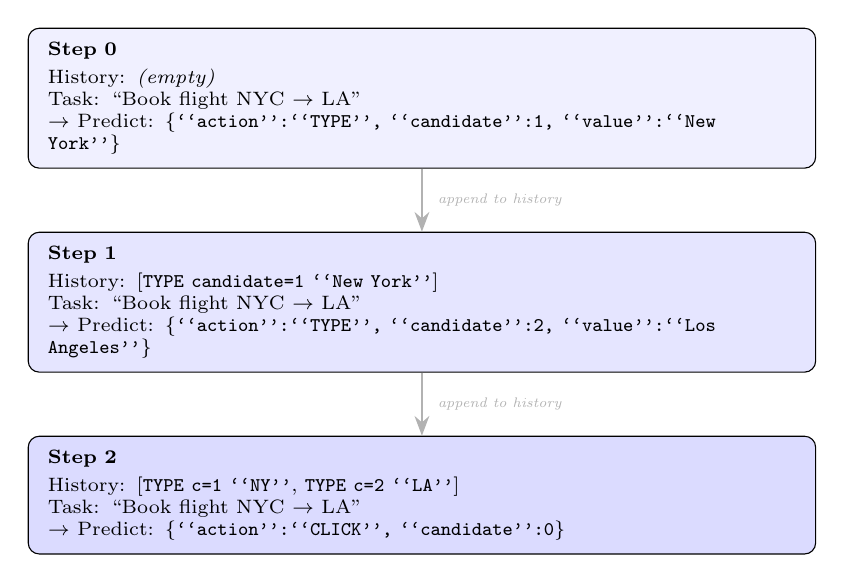
\begin{tikzpicture}[
  step/.style={rectangle, draw, rounded corners=4pt,
               minimum width=10cm, minimum height=1.4cm,
               text width=9.5cm, font=\scriptsize,
               inner sep=5pt, fill=#1},
  step/.default={blue!6},
  arrow/.style={-{Stealth[length=2.5mm]}, thick, color=gray!60},
  lbl/.style={font=\tiny\itshape\color{gray!70!black}, right=2pt}
]
  % Step 0
  \node[step=blue!6] (s0) {
    \textbf{Step 0} \\[2pt]
    History: \emph{(empty)} \\
    Task: ``Book flight NYC $\rightarrow$ LA'' \\
    $\rightarrow$ Predict: \texttt{\{``action'':``TYPE'', ``candidate'':1, ``value'':``New York''\}}
  };

  % Step 1
  \node[step=blue!10, below=0.8cm of s0] (s1) {
    \textbf{Step 1} \\[2pt]
    History: [\texttt{TYPE candidate=1 ``New York''}] \\
    Task: ``Book flight NYC $\rightarrow$ LA'' \\
    $\rightarrow$ Predict: \texttt{\{``action'':``TYPE'', ``candidate'':2, ``value'':``Los Angeles''\}}
  };

  % Step 2
  \node[step=blue!14, below=0.8cm of s1] (s2) {
    \textbf{Step 2} \\[2pt]
    History: [\texttt{TYPE c=1 ``NY''}, \texttt{TYPE c=2 ``LA''}] \\
    Task: ``Book flight NYC $\rightarrow$ LA'' \\
    $\rightarrow$ Predict: \texttt{\{``action'':``CLICK'', ``candidate'':0\}}
  };

  % Arrows
  \draw[arrow] (s0.south) -- node[lbl]{append to history} (s1.north);
  \draw[arrow] (s1.south) -- node[lbl]{append to history} (s2.north);
\end{tikzpicture}
\caption{Teacher forcing: cumulative action history injected at each step.}
\label{fig:teacher-forcing}
\end{figure}


%% ================================================================
\section{Candidate Selection Pipeline}
%% ================================================================

The candidate selection pipeline transforms a raw DOM into a compact,
shuffled list of 64 elements that the model can reference by index
(Figure~\ref{fig:candidate-pipeline}).

\begin{figure}[H]
\centering
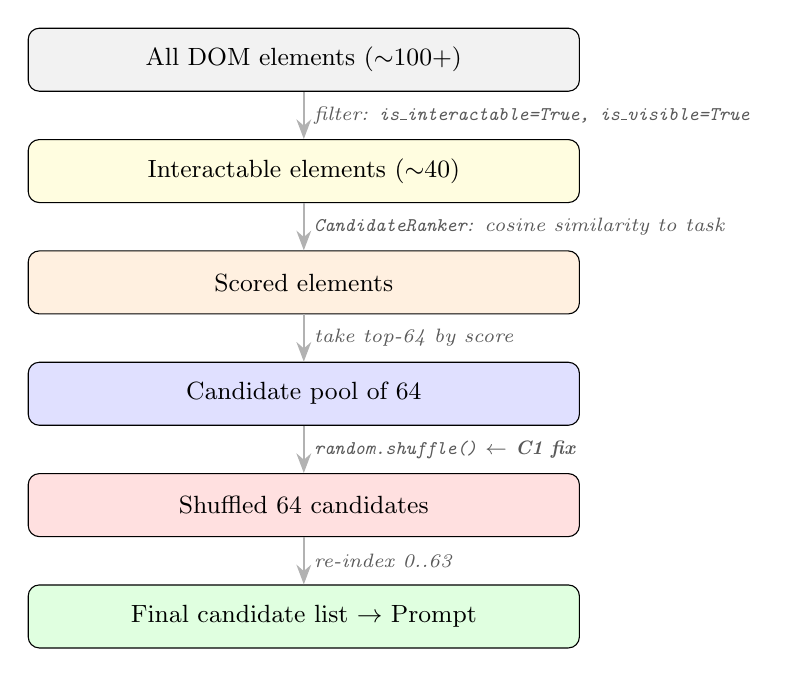
\begin{tikzpicture}[
  block/.style={rectangle, draw, rounded corners=4pt,
                minimum width=7cm, minimum height=0.8cm,
                text centered, font=\small, fill=#1, inner sep=4pt},
  block/.default={blue!8},
  arrow/.style={-{Stealth[length=2.5mm]}, thick, color=gray!60},
  note/.style={font=\scriptsize\itshape, color=gray!70!black},
  node distance=0.6cm
]
  \node[block=gray!10] (dom) {All DOM elements ($\sim$100+)};
  \node[block=yellow!12, below=of dom] (filt) {Interactable elements ($\sim$40)};
  \node[block=orange!12, below=of filt] (scored) {Scored elements};
  \node[block=blue!12, below=of scored] (pool) {Candidate pool of 64};
  \node[block=red!12, below=of pool] (shuf) {Shuffled 64 candidates};
  \node[block=green!12, below=of shuf] (final) {Final candidate list $\rightarrow$ Prompt};

  \draw[arrow] (dom) -- node[right, note]{filter: \texttt{is\_interactable=True, is\_visible=True}} (filt);
  \draw[arrow] (filt) -- node[right, note]{\texttt{CandidateRanker}: cosine similarity to task} (scored);
  \draw[arrow] (scored) -- node[right, note]{take top-64 by score} (pool);
  \draw[arrow] (pool) -- node[right, note]{\texttt{random.shuffle()} $\leftarrow$ \textbf{C1 fix}} (shuf);
  \draw[arrow] (shuf) -- node[right, note]{re-index 0..63} (final);
\end{tikzpicture}
\caption{Candidate selection pipeline from raw DOM to prompt-ready list.}
\label{fig:candidate-pipeline}
\end{figure}


\subsection{Candidate Prompt Format (I4~Fix)}

Figure~\ref{fig:candidate-format} shows the candidate format before
and after the I4~bounding box restoration.

\begin{figure}[H]
\centering
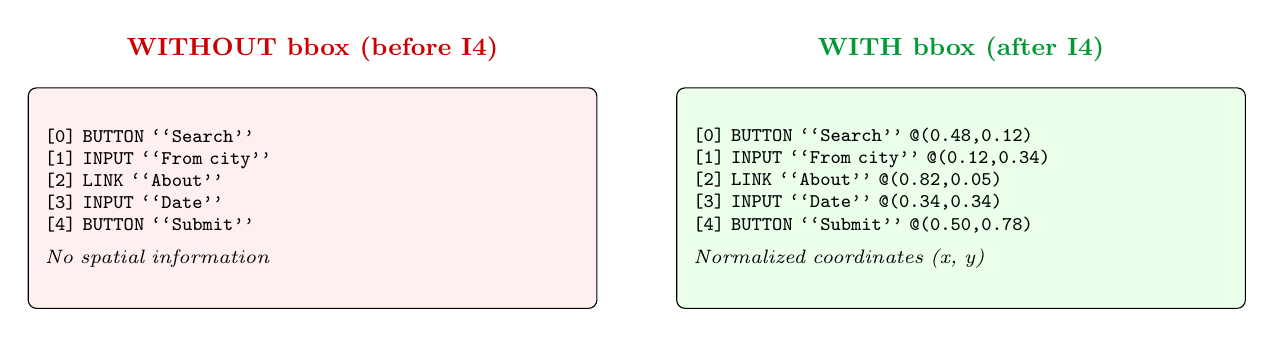
\begin{tikzpicture}[
  box/.style={rectangle, draw, rounded corners=3pt,
              text width=6.8cm, minimum height=2.8cm,
              font=\ttfamily\scriptsize, inner sep=6pt, fill=#1,
              align=left},
  title/.style={font=\small\bfseries}
]
  % Left box — without bbox
  \node[box=red!6] (before) {
    {[0]} BUTTON ``Search'' \\
    {[1]} INPUT ``From city'' \\
    {[2]} LINK ``About'' \\
    {[3]} INPUT ``Date'' \\
    {[4]} BUTTON ``Submit'' \\[4pt]
    \textrm{\itshape\scriptsize No spatial information}
  };
  \node[title, above=0.2cm of before, text=critical] {WITHOUT bbox (before I4)};

  % Right box — with bbox
  \node[box=green!8, right=1.0cm of before] (after) {
    {[0]} BUTTON ``Search'' @(0.48,0.12) \\
    {[1]} INPUT ``From city'' @(0.12,0.34) \\
    {[2]} LINK ``About'' @(0.82,0.05) \\
    {[3]} INPUT ``Date'' @(0.34,0.34) \\
    {[4]} BUTTON ``Submit'' @(0.50,0.78) \\[4pt]
    \textrm{\itshape\scriptsize Normalized coordinates (x, y)}
  };
  \node[title, above=0.2cm of after, text=improvement] {WITH bbox (after I4)};
\end{tikzpicture}
\caption{Candidate prompt format comparison: spatial grounding via bounding boxes.}
\label{fig:candidate-format}
\end{figure}


%% ================================================================
\section{Critical Defects (C1--C4)}
%% ================================================================

\subsection{C1: Train/Inference Candidate Distribution Mismatch}

\begin{description}[leftmargin=2cm,style=nextline]
\item[Severity] \textcolor{critical}{Critical}
\item[File] \texttt{inference/run\_agent.py}
\item[Root Cause]
  During training, \texttt{mind2web\_loader.py} shuffles candidates randomly.
  At inference, \texttt{\_build\_candidates\_from\_state()} sorted candidates
  by word-overlap score (highest first), creating a systematic distribution
  mismatch.
\item[Fix]
  After scoring and limiting to the top~$N$, apply
  \texttt{random.shuffle(candidates)} and re-index.
  See Figure~\ref{fig:candidate-pipeline} for placement in the pipeline.
\end{description}


\subsection{C2: Stage 2 Trajectories Are Single-Step}

\begin{description}[leftmargin=2cm,style=nextline]
\item[Severity] \textcolor{critical}{Critical}
\item[Files] \texttt{data/mind2web\_loader.py}, \texttt{training/train\_supervised.py}
\item[Root Cause]
  \texttt{build\_trajectories()} grouped by \texttt{annotation\_id}
  (unique per sample), producing single-step ``trajectories.''
\item[Fix]
  Group by \texttt{hash(confirmed\_task + website + action\_reprs)}.
  See Figures~\ref{fig:traj-grouping} and~\ref{fig:teacher-forcing}.
\end{description}


\subsection{C3: Candidate Count Mismatch}

\begin{description}[leftmargin=2cm,style=nextline]
\item[Severity] \textcolor{critical}{Critical}
\item[Files] 5 files (config, loader, prompt builder, agent)
\item[Root Cause]
  Candidate counts were inconsistent: loader=30, prompt builder=50,
  inference=20.
\item[Fix]
  Standardized to 64 total (1 positive + 63 negatives).
\end{description}


\subsection{C4: Evaluation Metric Measures Noise}

\begin{description}[leftmargin=2cm,style=nextline]
\item[Severity] \textcolor{critical}{Critical}
\item[Files] \texttt{evaluation/evaluate.py}, \texttt{data/mind2web\_loader.py}
\item[Root Cause]
  Evaluator compared predicted and ground-truth candidate \emph{indices}
  directly, but candidates are randomly shuffled each time.
\item[Fix]
  Added \texttt{gt\_backend\_node\_id} to samples. Compare by stable
  element identity. Renamed metric to \texttt{element\_accuracy}.
\end{description}


%% ================================================================
\section{Fixed Evaluation Pipeline (C4)}
%% ================================================================

Figure~\ref{fig:eval-pipeline} shows the evaluation comparison
before and after the C4~fix.

\begin{figure}[H]
\centering
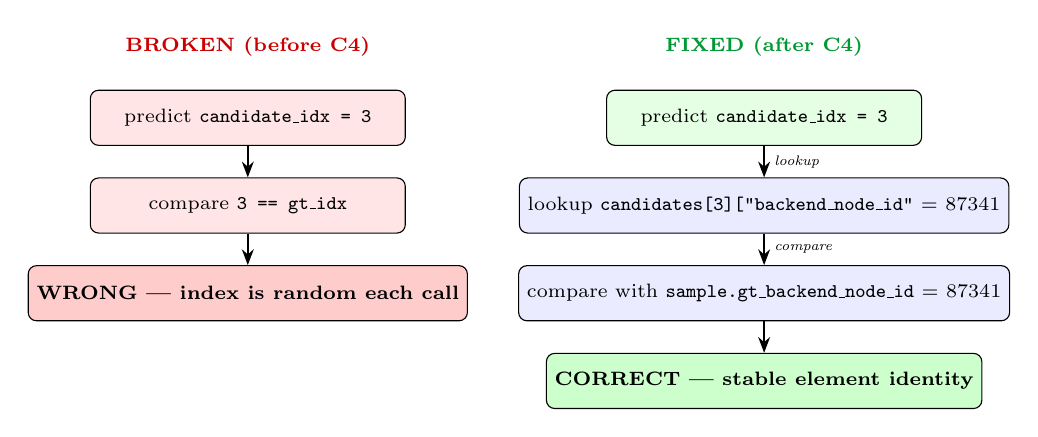
\begin{tikzpicture}[
  box/.style={rectangle, draw, rounded corners=3pt,
              minimum width=4cm, minimum height=0.7cm,
              text centered, font=\scriptsize, fill=#1, inner sep=3pt},
  arrow/.style={-{Stealth[length=2mm]}, thick},
  lbl/.style={font=\scriptsize\bfseries},
  node distance=0.4cm
]
  % ── BROKEN pipeline ──
  \node[lbl, text=critical] (bt) {BROKEN (before C4)};
  \node[box=red!10, below=0.3cm of bt] (bp) {predict \texttt{candidate\_idx = 3}};
  \node[box=red!10, below=of bp] (bc) {compare \texttt{3 == gt\_idx}};
  \node[box=red!20, below=of bc, font=\scriptsize\bfseries] (br) {WRONG --- index is random each call};

  \draw[arrow] (bp) -- (bc);
  \draw[arrow] (bc) -- (br);

  % ── FIXED pipeline ──
  \node[lbl, text=improvement, right=3.5cm of bt] (ft) {FIXED (after C4)};
  \node[box=green!10, below=0.3cm of ft] (fp) {predict \texttt{candidate\_idx = 3}};
  \node[box=blue!8, below=of fp] (fl) {lookup \texttt{candidates[3]["backend\_node\_id"} = 87341};
  \node[box=blue!8, below=of fl] (fc) {compare with \texttt{sample.gt\_backend\_node\_id} = 87341};
  \node[box=green!20, below=of fc, font=\scriptsize\bfseries] (fr) {CORRECT --- stable element identity};

  \draw[arrow] (fp) -- node[right, font=\tiny\itshape]{lookup} (fl);
  \draw[arrow] (fl) -- node[right, font=\tiny\itshape]{compare} (fc);
  \draw[arrow] (fc) -- (fr);
\end{tikzpicture}
\caption{Evaluation pipeline: broken index comparison vs fixed identity comparison.}
\label{fig:eval-pipeline}
\end{figure}


%% ================================================================
\section{LoRA Adapter Injection}
%% ================================================================

The VLA model uses QLoRA~(4-bit NormalFloat quantization) with
low-rank adapters injected into the frozen base weights
(Figure~\ref{fig:lora}).

The update rule is:
\[
  W' = W + \frac{\alpha}{r}\, B A
  \qquad\text{where}\quad
  B \in \mathbb{R}^{d \times r},\;
  A \in \mathbb{R}^{r \times k}
\]

with $r = 16$, $\alpha = 32$, and dropout $= 0.05$.

\begin{figure}[H]
\centering
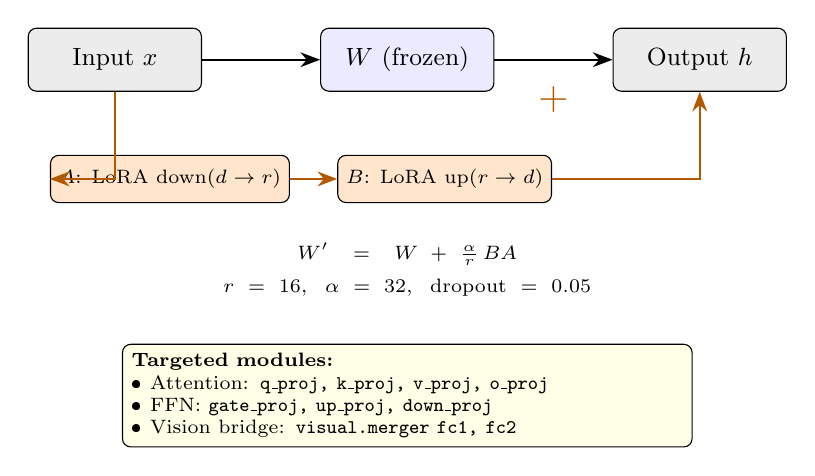
\begin{tikzpicture}[
  block/.style={rectangle, draw, rounded corners=3pt,
                minimum height=0.8cm, minimum width=2.2cm,
                text centered, font=\small, inner sep=3pt, fill=#1},
  block/.default={blue!10},
  arrow/.style={-{Stealth[length=2.5mm]}, thick},
  lorablock/.style={rectangle, draw, rounded corners=3pt,
                    minimum height=0.6cm, minimum width=1.6cm,
                    text centered, font=\scriptsize, inner sep=3pt, fill=#1},
  node distance=0.5cm
]
  % Main path
  \node[block=gray!15] (input) {Input $x$};
  \node[block=blue!8, right=1.5cm of input] (W) {$W$ (frozen)};
  \node[block=gray!15, right=1.5cm of W] (output) {Output $h$};

  \draw[arrow] (input) -- (W);
  \draw[arrow] (W) -- (output);

  % LoRA bypass
  \node[lorablock=orange!20, below=0.8cm of input, xshift=0.7cm] (A) {$A$: LoRA down\\($d \rightarrow r$)};
  \node[lorablock=orange!20, right=0.6cm of A] (B) {$B$: LoRA up\\($r \rightarrow d$)};

  \draw[arrow, color=orange!70!black] (input.south) |- (A.west);
  \draw[arrow, color=orange!70!black] (A) -- (B);
  \draw[arrow, color=orange!70!black] (B.east) -| (output.south);

  % Plus sign
  \node[font=\Large\bfseries, color=orange!70!black]
    at ($(W)!0.5!(output) + (0,-0.5)$) {$+$};

  % Formula
  \node[font=\scriptsize, below=1.8cm of W, text width=6cm, align=center]
    {$W' = W + \frac{\alpha}{r}\, BA$\\[4pt]
     $r=16,\;\alpha=32,\;\text{dropout}=0.05$};

  % Target modules list
  \node[rectangle, draw, rounded corners=3pt, fill=yellow!10,
        font=\scriptsize, text width=7cm, align=left,
        below=3.2cm of W] (targets) {
    \textbf{Targeted modules:}\\
    \textbullet\ Attention: \texttt{q\_proj, k\_proj, v\_proj, o\_proj}\\
    \textbullet\ FFN: \texttt{gate\_proj, up\_proj, down\_proj}\\
    \textbullet\ Vision bridge: \texttt{visual.merger} \texttt{fc1, fc2}
  };
\end{tikzpicture}
\caption{QLoRA adapter injection into a transformer block.}
\label{fig:lora}
\end{figure}


%% ================================================================
\section{Significant Defects (S1--S7)}
%% ================================================================

\subsection{S1: Missing LR Scheduler}

\begin{description}[leftmargin=2cm,style=nextline]
\item[File] \texttt{training/train\_supervised.py}
\item[Fix]
  Added \texttt{get\_cosine\_schedule\_with\_warmup}. Warmup ratio = 0.1.
  Scheduler stepped after every optimizer update. Current LR logged.
\end{description}

\subsection{S2: Uncertainty Uses Wrong Key for Beam Agreement}

\begin{description}[leftmargin=2cm,style=nextline]
\item[File] \texttt{models/uncertainty.py}
\item[Fix]
  Changed signature from \texttt{a.get('element\_id')} to
  \texttt{a.get('candidate')}.
\end{description}

\subsection{S3: Failure Detector Blind to Candidate Actions}

\begin{description}[leftmargin=2cm,style=nextline]
\item[File] \texttt{memory/failure\_detector.py}
\item[Fix]
  Included \texttt{candidate} key in \texttt{\_action\_signature()}.
\end{description}

\subsection{S4: Screenshot Placeholder Creates Spurious Pattern}

\begin{description}[leftmargin=2cm,style=nextline]
\item[File] \texttt{data/mind2web\_loader.py}
\item[Fix]
  Return \texttt{None} instead of 224$\times$224 white image. Collate
  function skips \texttt{None} screenshots.
\end{description}

\subsection{S5: Prompt Instruction Contradiction}

\begin{description}[leftmargin=2cm,style=nextline]
\item[File] \texttt{models/prompt\_builder.py}
\item[Fix]
  Removed ``Think about the best element to interact with.''
\end{description}

\subsection{S6: Scroll Attempts Persist Across Tasks}

\begin{description}[leftmargin=2cm,style=nextline]
\item[File] \texttt{inference/run\_agent.py}
\item[Fix]
  Initialized \texttt{\_scroll\_attempts = 0} in \texttt{\_\_init\_\_()}
  and reset at start of \texttt{run\_task()}.
\end{description}

\subsection{S7: Fragile Element Lookup via Sequential Counter}

\begin{description}[leftmargin=2cm,style=nextline]
\item[File] \texttt{environment/playwright\_env.py}
\item[Fix]
  Try \texttt{data-backend-node-id} attribute selector first; fall back
  to sequential TreeWalker traversal.
\end{description}


%% ================================================================
\section{Full Inference Loop}
%% ================================================================

Figure~\ref{fig:inference-loop} shows the complete
\texttt{run\_task()} execution flow.

\begin{figure}[H]
\centering
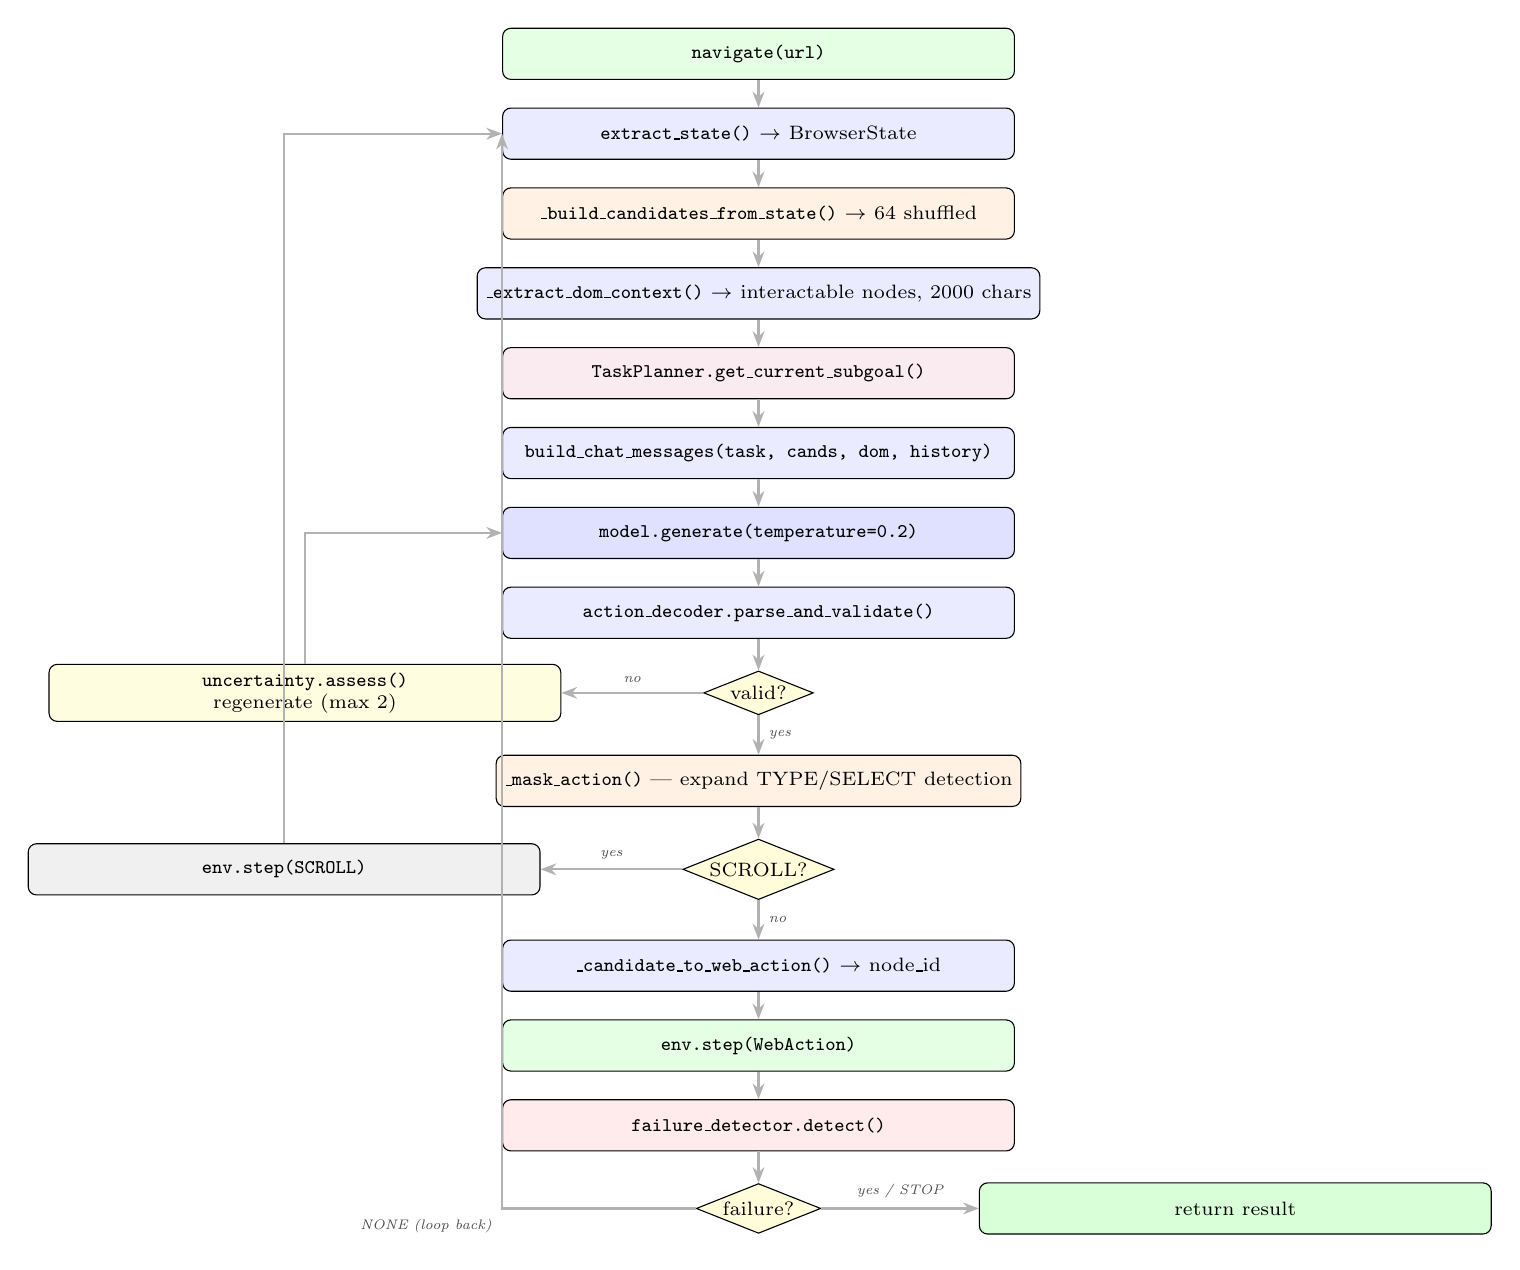
\begin{tikzpicture}[
  block/.style={rectangle, draw, rounded corners=3pt,
                minimum width=6.5cm, minimum height=0.65cm,
                text centered, font=\scriptsize, fill=#1, inner sep=3pt},
  block/.default={blue!8},
  decision/.style={diamond, draw, aspect=2.5, inner sep=1pt,
                   font=\scriptsize, fill=yellow!15},
  arrow/.style={-{Stealth[length=2mm]}, thick, color=gray!60},
  note/.style={font=\tiny\itshape, color=gray!60!black},
  node distance=0.35cm
]
  \node[block=green!10] (nav)   {\texttt{navigate(url)}};
  \node[block, below=of nav] (ext)   {\texttt{extract\_state()} $\rightarrow$ BrowserState};
  \node[block=orange!10, below=of ext] (cand) {\texttt{\_build\_candidates\_from\_state()} $\rightarrow$ 64 shuffled};
  \node[block, below=of cand] (dom)  {\texttt{\_extract\_dom\_context()} $\rightarrow$ interactable nodes, 2000 chars};
  \node[block=purple!8, below=of dom] (plan) {\texttt{TaskPlanner.get\_current\_subgoal()}};
  \node[block, below=of plan] (msg)  {\texttt{build\_chat\_messages(task, cands, dom, history)}};
  \node[block=blue!12, below=of msg] (gen) {\texttt{model.generate(temperature=0.2)}};
  \node[block, below=of gen] (parse) {\texttt{action\_decoder.parse\_and\_validate()}};

  \node[decision, below=0.4cm of parse] (valid) {valid?};
  \node[block=yellow!12, left=1.8cm of valid, text width=2.8cm] (regen) {
    \texttt{uncertainty.assess()}\\regenerate (max~2)
  };

  \node[block=orange!10, below=0.5cm of valid] (mask) {\texttt{\_mask\_action()} --- expand TYPE/SELECT detection};

  \node[decision, below=0.4cm of mask] (scroll) {SCROLL?};
  \node[block=gray!12, left=1.8cm of scroll, text width=2.4cm] (scrollex) {\texttt{env.step(SCROLL)}};

  \node[block, below=0.5cm of scroll] (map) {\texttt{\_candidate\_to\_web\_action()} $\rightarrow$ node\_id};
  \node[block=green!10, below=of map] (exec) {\texttt{env.step(WebAction)}};
  \node[block=red!8, below=of exec] (fail) {\texttt{failure\_detector.detect()}};

  \node[decision, below=0.4cm of fail] (failq) {failure?};
  \node[block=green!15, right=2.0cm of failq, text width=1.8cm] (ret) {return result};

  % Arrows
  \draw[arrow] (nav) -- (ext);
  \draw[arrow] (ext) -- (cand);
  \draw[arrow] (cand) -- (dom);
  \draw[arrow] (dom) -- (plan);
  \draw[arrow] (plan) -- (msg);
  \draw[arrow] (msg) -- (gen);
  \draw[arrow] (gen) -- (parse);
  \draw[arrow] (parse) -- (valid);

  \draw[arrow] (valid) -- node[above, note]{no} (regen);
  \draw[arrow] (regen.north) |- (gen.west);
  \draw[arrow] (valid) -- node[right, note]{yes} (mask);

  \draw[arrow] (mask) -- (scroll);
  \draw[arrow] (scroll) -- node[above, note]{yes} (scrollex);
  \draw[arrow] (scrollex.north) |- (ext.west);
  \draw[arrow] (scroll) -- node[right, note]{no} (map);

  \draw[arrow] (map) -- (exec);
  \draw[arrow] (exec) -- (fail);
  \draw[arrow] (fail) -- (failq);
  \draw[arrow] (failq) -- node[above, note]{yes / STOP} (ret);
  \draw[arrow] (failq.west) -| node[below left, note]{NONE (loop back)} (ext.west |- failq.west) -- (ext.west);
\end{tikzpicture}
\caption{Full inference loop: \texttt{run\_task()} execution flow.}
\label{fig:inference-loop}
\end{figure}


%% ================================================================
\section{Moderate Defects (M1--M2)}
%% ================================================================

\subsection{M1: No Task-Level Success Metric}

\begin{description}[leftmargin=2cm,style=nextline]
\item[File] \texttt{evaluation/evaluate.py}
\item[Fix]
  Added \texttt{evaluate\_trajectory()} method. A task succeeds only if
  \emph{all} steps have \texttt{full\_match=True}.
  \texttt{task\_success\_rate} is in \texttt{compute\_metrics()}.
\end{description}

\subsection{M2: Action Masking Too Aggressive for TYPE}

\begin{description}[leftmargin=2cm,style=nextline]
\item[File] \texttt{inference/run\_agent.py}
\item[Fix]
  Expanded typeable detection to include
  \texttt{role="textbox"}, \texttt{role="searchbox"},
  \texttt{role="combobox"}, and \texttt{contenteditable="true"}.
\end{description}


%% ================================================================
\section{Architectural Improvements}
%% ================================================================

\subsection{I1: Include Serialized DOM in Model Input}

Added \texttt{dom\_context} parameter to prompt building methods.
A ``\texttt{[DOM Context]}'' section is appended after the candidate
list.

\subsection{I2: Embedding-Based Candidate Ranking}

\texttt{CandidateRanker} uses \texttt{all-MiniLM-L6-v2} for cosine
similarity. Falls back to word overlap if unavailable.

Figure~\ref{fig:semantic-ranking} shows the advantage of semantic
ranking over word overlap.

\begin{figure}[H]
\centering
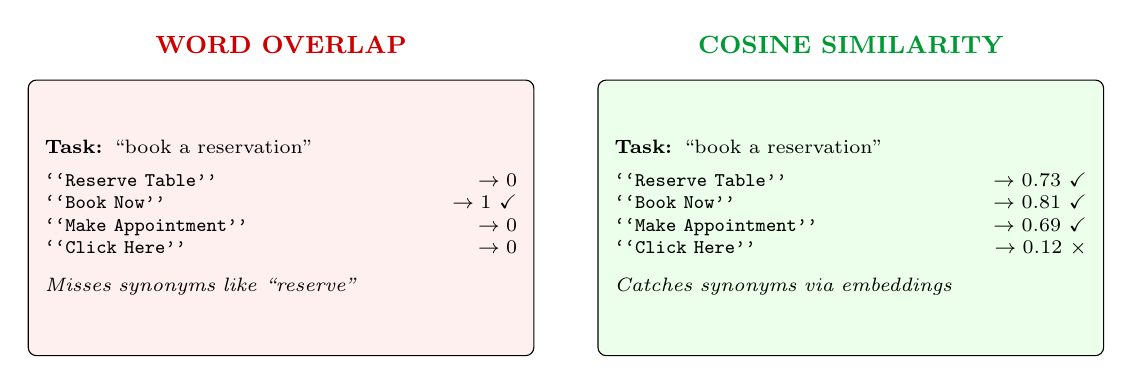
\begin{tikzpicture}[
  col/.style={rectangle, draw, rounded corners=3pt,
              text width=6.0cm, minimum height=3.5cm,
              font=\scriptsize, inner sep=6pt, fill=#1, align=left},
  title/.style={font=\small\bfseries},
]
  % Left
  \node[col=red!6] (wl) {
    \textbf{Task:} ``book a reservation''\\[4pt]
    \texttt{``Reserve Table''}\hfill$\rightarrow 0$\\
    \texttt{``Book Now''}\hfill$\rightarrow 1$ \checkmark\\
    \texttt{``Make Appointment''}\hfill$\rightarrow 0$\\
    \texttt{``Click Here''}\hfill$\rightarrow 0$\\[6pt]
    \emph{Misses synonyms like ``reserve''}
  };
  \node[title, above=0.2cm of wl, text=critical] {WORD OVERLAP};

  % Right
  \node[col=green!8, right=0.8cm of wl] (cs) {
    \textbf{Task:} ``book a reservation''\\[4pt]
    \texttt{``Reserve Table''}\hfill$\rightarrow 0.73$ \checkmark\\
    \texttt{``Book Now''}\hfill$\rightarrow 0.81$ \checkmark\\
    \texttt{``Make Appointment''}\hfill$\rightarrow 0.69$ \checkmark\\
    \texttt{``Click Here''}\hfill$\rightarrow 0.12$ $\times$\\[6pt]
    \emph{Catches synonyms via embeddings}
  };
  \node[title, above=0.2cm of cs, text=improvement] {COSINE SIMILARITY};
\end{tikzpicture}
\caption{Semantic ranking vs word overlap: synonym detection.}
\label{fig:semantic-ranking}
\end{figure}


\subsection{I3: Increase Candidate Limit to 64}

Unified candidate limit across all components.
Figure~\ref{fig:pool-recall} shows the estimated relationship between
pool size and target element recall.

\begin{figure}[H]
\centering
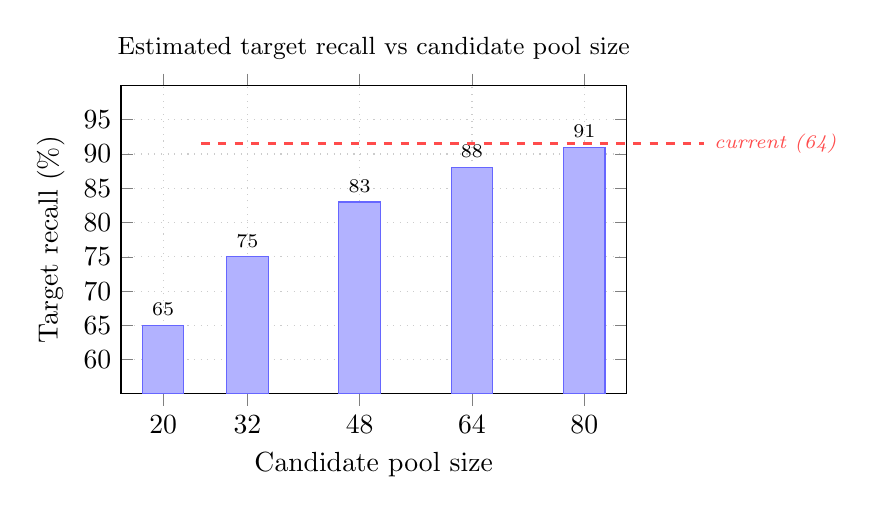
\begin{tikzpicture}
\begin{axis}[
  width=8cm, height=5.5cm,
  ybar,
  bar width=15pt,
  xlabel={Candidate pool size},
  ylabel={Target recall (\%)},
  ymin=55, ymax=100,
  xtick={20,32,48,64,80},
  ytick={60,65,70,75,80,85,90,95},
  nodes near coords,
  nodes near coords align={vertical},
  every node near coord/.style={font=\scriptsize},
  title={\small Estimated target recall vs candidate pool size},
  grid=major,
  grid style={dotted, gray!40},
]
  \addplot[fill=blue!30, draw=blue!60] coordinates {
    (20, 65) (32, 75) (48, 83) (64, 88) (80, 91)
  };
\end{axis}

% Dashed line at y=88
\draw[dashed, thick, red!70] (1.02,3.18) -- (7.4,3.18)
  node[right, font=\scriptsize\itshape, text=red!70] {current (64)};
\end{tikzpicture}
\caption{Estimated target recall vs candidate pool size.}
\label{fig:pool-recall}
\end{figure}


\subsection{I4: Restore Spatial Grounding via Bounding Boxes}

See Figure~\ref{fig:candidate-format} for the format comparison.
Candidates now carry \texttt{bounding\_box\_rect} from Mind2Web and
live \texttt{getBoundingClientRect()} at inference.


\subsection{I5: Add a Planning Layer}

\texttt{TaskPlanner} decomposes high-level tasks into subgoals that
are injected into the prompt (Figure~\ref{fig:planning-layer}).

\begin{figure}[H]
\centering
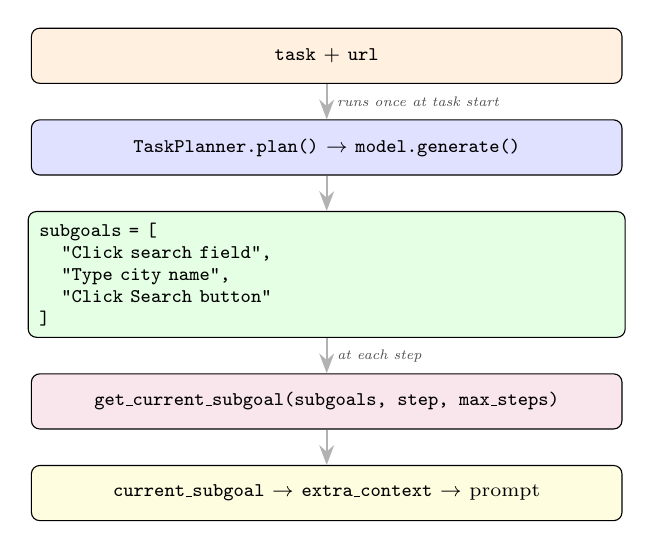
\begin{tikzpicture}[
  block/.style={rectangle, draw, rounded corners=3pt,
                minimum width=7.5cm, minimum height=0.7cm,
                text centered, font=\scriptsize, fill=#1, inner sep=4pt},
  block/.default={blue!8},
  arrow/.style={-{Stealth[length=2.5mm]}, thick, color=gray!60},
  note/.style={font=\tiny\itshape, color=gray!60!black},
  node distance=0.45cm
]
  \node[block=orange!12] (input) {\texttt{task} + \texttt{url}};
  \node[block=blue!12, below=of input] (plan) {\texttt{TaskPlanner.plan()} $\rightarrow$ \texttt{model.generate()}};
  \node[block=green!10, below=of plan, text width=7.3cm, align=left] (goals) {
    \texttt{subgoals = [}\\
    \quad \texttt{"Click search field",}\\
    \quad \texttt{"Type city name",}\\
    \quad \texttt{"Click Search button"}\\
    \texttt{]}
  };
  \node[block=purple!10, below=of goals] (get) {\texttt{get\_current\_subgoal(subgoals, step, max\_steps)}};
  \node[block=yellow!12, below=of get] (ctx) {\texttt{current\_subgoal} $\rightarrow$ \texttt{extra\_context} $\rightarrow$ prompt};

  \draw[arrow] (input) -- node[right, note]{runs once at task start} (plan);
  \draw[arrow] (plan) -- (goals);
  \draw[arrow] (goals) -- node[right, note]{at each step} (get);
  \draw[arrow] (get) -- (ctx);
\end{tikzpicture}
\caption{Planning layer: task decomposition into subgoals.}
\label{fig:planning-layer}
\end{figure}


\subsection{I6: Increase Vision Resolution}

Increased \texttt{image\_max\_pixels} from 401,408 to 802,816
($\approx 896 \times 896$). Added runtime warning when total vision
token count exceeds 5,000.


%% ================================================================
\section{Configuration Alignment}
%% ================================================================

\begin{table}[H]
\centering
\caption{Key configuration parameters (before $\rightarrow$ after)}
\begin{tabular}{lcc}
\toprule
\textbf{Parameter} & \textbf{Before} & \textbf{After} \\
\midrule
\texttt{max\_neg\_candidates}  & 30                                         & 63      \\
\texttt{max\_candidates}       & 50 / 20                                    & 64      \\
\texttt{image\_max\_pixels}    & 401,408                                    & 802,816 \\
\texttt{stage2\_epochs}        & 3                                          & 5       \\
\texttt{scroll\_aug\_ratio}    & 0.05 (yaml) / 0.2 (code) --- inconsistent & 0.05    \\
\texttt{warmup\_ratio}         & 0.1 (unused)                               & 0.1     \\
LR Scheduler                   & None                                       & Cosine  \\
\bottomrule
\end{tabular}
\end{table}


%% ================================================================
\section{Verification}
%% ================================================================

\subsection{Compilation Check}

All 11 modified Python source files pass syntactic compilation via
\texttt{python3 -m py\_compile}:

\begin{verbatim}
OK config.py             OK candidate_ranker.py
OK uncertainty.py        OK task_planner.py
OK failure_detector.py   OK mind2web_loader.py
OK prompt_builder.py     OK evaluate.py
OK playwright_env.py     OK run_agent.py
OK train_supervised.py
\end{verbatim}

\subsection{Backward Compatibility}

\begin{itemize}
\item All function signatures maintain their original default arguments.
\item New parameters (\texttt{dom\_context}, \texttt{gt\_backend\_node\_id})
  default to empty/negative values.
\item New files (\texttt{candidate\_ranker.py}, \texttt{task\_planner.py})
  are optional, imported lazily.
\end{itemize}


%% ================================================================
\section{Conclusion}
%% ================================================================

This audit resolved all 19 identified defects and improvements across
12 source files. The most impactful changes were:

\begin{enumerate}
\item \textbf{C1/C2}: Restoring distribution alignment between training
  and inference (candidate shuffling + trajectory grouping).
\item \textbf{C4}: Switching evaluation from noisy index comparison to
  stable element identity matching.
\item \textbf{S1}: Adding a cosine LR scheduler to prevent
  overfitting in later training epochs.
\item \textbf{I3/I4}: Expanding the candidate window to 64 with spatial
  bounding box grounding.
\end{enumerate}


\end{document}
